\documentclass{article} % For LaTeX2e
\usepackage{iclr2026_conference,times}

% Optional math commands from https://github.com/goodfeli/dlbook_notation.
\input{math_commands.tex}

\usepackage{hyperref}
\usepackage{url}

\usepackage{amsmath}
\usepackage{amssymb}
\usepackage{booktabs}
\usepackage{graphicx}
\usepackage{subcaption}
\usepackage{xcolor}
\usepackage{xspace}
\usepackage{algorithm}
\usepackage{algpseudocode}

% Paper-specific notation. Loaded after math_commands.tex; all names are
% prefixed or distinctive so nothing in the dlbook notation is redefined.

% --- proposal / verification counts -----------------------------------------
\newcommand{\nprop}{N_{\mathrm{prop}}}       % proposed tokens per model call
\newcommand{\ncorrect}{N_{\mathrm{cor}}}     % longest correct prefix
\newcommand{\naccepted}{N_{\mathrm{acc}}}    % committed tokens = Ncor + 1
\newcommand{\budget}{C}                      % node budget per call

% --- sampling ----------------------------------------------------------------
\newcommand{\Pick}{\operatorname{Pick}}
\newcommand{\aux}{u}                         % auxiliary variable u ~ U[0,1]
\newcommand{\auxs}{\mathbf{u}}
\newcommand{\base}{Q_\phi}                   % base / reference AR model
\newcommand{\prop}{P_\theta}                 % proposal (PTP) model
\newcommand{\accept}{\mathcal{A}}            % acceptance set

% --- branching model ---------------------------------------------------------
\newcommand{\pizero}{\pi_0}                  % zero-inflation probability
\newcommand{\rhoc}{\rho}                     % intra-generation correlation
\newcommand{\frail}{\Theta}                  % per-generation frailty
\newcommand{\Sfun}{S}                        % survival table S[w,d]
\newcommand{\alive}{S}                       % strands alive
\newcommand{\extinct}{T}                     % extinction time
\newcommand{\width}{W}                       % width profile W(d)
\newcommand{\capt}{d_{\max}}                 % structural proposal-length cap
\newcommand{\BetaBin}{\mathrm{BetaBin}}

% --- misc --------------------------------------------------------------------
\newcommand{\ie}{i.e.\@\xspace}
\newcommand{\eg}{e.g.\@\xspace}
\newcommand{\todo}[1]{\textcolor{red}{[#1]}}


\graphicspath{{fig/}{fig/slides/}}

\title{Elucidating Inference in Multi-Token Prediction:\\
Proposal, Verification, and Parallelization}

% Authors must not appear in the submitted version. They should be hidden
% as long as the \iclrfinalcopy macro remains commented out below.
% Non-anonymous submissions will be rejected without review.
%
% TODO(draft): confirm the final author list and affiliations before submission.
\author{Justus Will\thanks{Correspondence: \texttt{jcwill@uci.edu}.} \\
Department of Computer Science\\
University of California, Irvine\\
Irvine, CA 92697, USA
}

\newcommand{\fix}{\marginpar{FIX}}
\newcommand{\new}{\marginpar{NEW}}

%\iclrfinalcopy % Uncomment for camera-ready version, but NOT for submission.
\begin{document}

\maketitle

\begin{abstract}
Multi-token prediction promises substantial inference speedups by emitting
several tokens per forward pass, but the quality of the resulting text depends
critically on how those tokens are accepted, rejected, or resampled. We study
this decoding layer directly, treating the multi-token model as a proposal
mechanism and asking what acceptance rule best trades throughput against
generation quality and alignment to an underlying autoregressive (AR) reference.
We organize the design space along three axes --- how proposals are
\emph{verified}, how many and how long the proposals are, and how proposal and
verification are \emph{parallelized} --- and we give a generative model of the
number of correct tokens per call that turns the second axis into an exactly
solvable allocation problem. Our experiments are conducted in PTP, a recent
multi-token inference framework, but the acceptance rules and the evaluation
protocol are framework-agnostic and apply to any model producing multiple tokens
per call. We report accepted-tokens-per-call, wall-clock speedup, and downstream
task quality across $62$ decoding configurations on Spec-Bench, and find that the
three measures order the rules differently: the rule that commits the most tokens
per call is frequently not the fastest, and is rarely the most faithful.
\end{abstract}

\section{Introduction}

Autoregressive decoding emits one token per forward pass. A multi-token model
breaks that constraint by proposing several tokens at once, but a proposal is not
an output: something must decide which of the proposed tokens are kept. That
decision --- the \emph{acceptance rule} --- is usually treated as a fixed
implementation detail, inherited from speculative
decoding~\citep{leviathan2023speculative,chen2023accelerating}, where it is
chosen to leave the base model's output distribution exactly intact. Once the
proposal mechanism is strong enough to offer many coherent tokens per call, that
choice stops being incidental. It sets the throughput, and it sets how far the
generated text drifts from what the base model would have produced.

This paper takes the decoding layer as the object of study. We ask the question
a practitioner actually faces: \emph{on a single GPU, what is the lowest latency
we can achieve that still produces high-quality outputs?} We organize the answer
along three axes.

\textbf{Verification.} What counts as a correct token? The strictest rule accepts
a proposed token only if the base model, driven by the same randomness, would have
emitted exactly that token. Relaxing it to ``the base model finds this token
plausible'' --- nucleus membership, a probability threshold, a likelihood ratio
--- accepts far more tokens per call, at a cost in faithfulness that we measure
rather than assume.

\textbf{Proposal geometry.} How many chances to take, and how long each should
be. Given a node budget, is it better to propose one long continuation, or fifty
short ones? We answer this by modelling the number of correct tokens per call as
the extinction time of a branching process, which makes the expected yield
separable across depth and the allocation problem exactly solvable.

\textbf{Parallelization.} Verification and the next proposal can run
concurrently if one speculates on the verification outcome. Partial Quadratic
Decoding (PQD)~\citep{draxler2025ptp} does this by preparing a branch for each
possible number of correct tokens and spending a budget across those branches. We
show that the branch weights and the value of a branch can be read off the same
calibrated model that solves the geometry problem, rather than estimated
separately.

Our contributions are: (i) a taxonomy and unified implementation of $12$ families
of acceptance rules for multi-token proposals, with a measurement protocol that
separates throughput from faithfulness (\S\ref{sec:acceptance}); (ii) a
zero-inflated Beta-Binomial branching model of $\ncorrect$ given proposal width
and context, which predicts per-call accepted-token histograms across three
orders of magnitude of width with $R^2 \geq 0.976$ (\S\ref{sec:model}); (iii) an
exact dynamic program for the resulting strand-length knapsack, and its
combination with PQD's budget allocation (\S\ref{sec:knapsack},
\S\ref{sec:pqd}); and (iv) an empirical study of $62$ decoding configurations
showing that accepted-tokens-per-call, wall-clock speedup, and faithfulness to
the base model order the rules differently (\S\ref{sec:experiments}).

\section{Background: multi-token proposals and their verification}
\label{sec:background}

\subsection{Auxiliary variables}

We build on Parallel Token Prediction (PTP)~\citep{draxler2025ptp}, which we
recap only as far as needed. A standard decoder predicts
$P_i := P(t_i \mid t_{<i})$ and then samples $t_i \sim P_i$. The sampling step is
where the sequential dependency lives, and it can be made explicit: drawing
$\aux_i \sim \mathcal{U}[0,1]$ and taking the inverse CDF,
\begin{equation}
  t_i = \Pick(\aux_i, P_i) \equiv \min\Big\{ j : \textstyle\sum_{l \leq j} P_{il} > \aux_i \Big\},
  \label{eq:pick}
\end{equation}
makes $t_i$ a \emph{deterministic} function of the context and the auxiliary
variable $\aux_i$. Since $\aux_i$ determines $t_i$ given $t_{<i}$, it carries the
same information as the token itself, so a model given
$\aux_i, \dots, \aux_k$ as inputs can predict $t_k$ without knowing the
intervening tokens. This is the basis of PTP: a model
$\prop(t_k \mid t_{<i}, \aux_i, \dots, \aux_k)$ emits many tokens in one call.
Figure~\ref{fig:auxiliaries} illustrates the shift of randomness from post-hoc
sampling to a random model input. We use the one-hot variant (O-PTP), whose
output probability for the proposed token doubles as a confidence estimate $c_k$.

\begin{figure}[t]
  \centering
  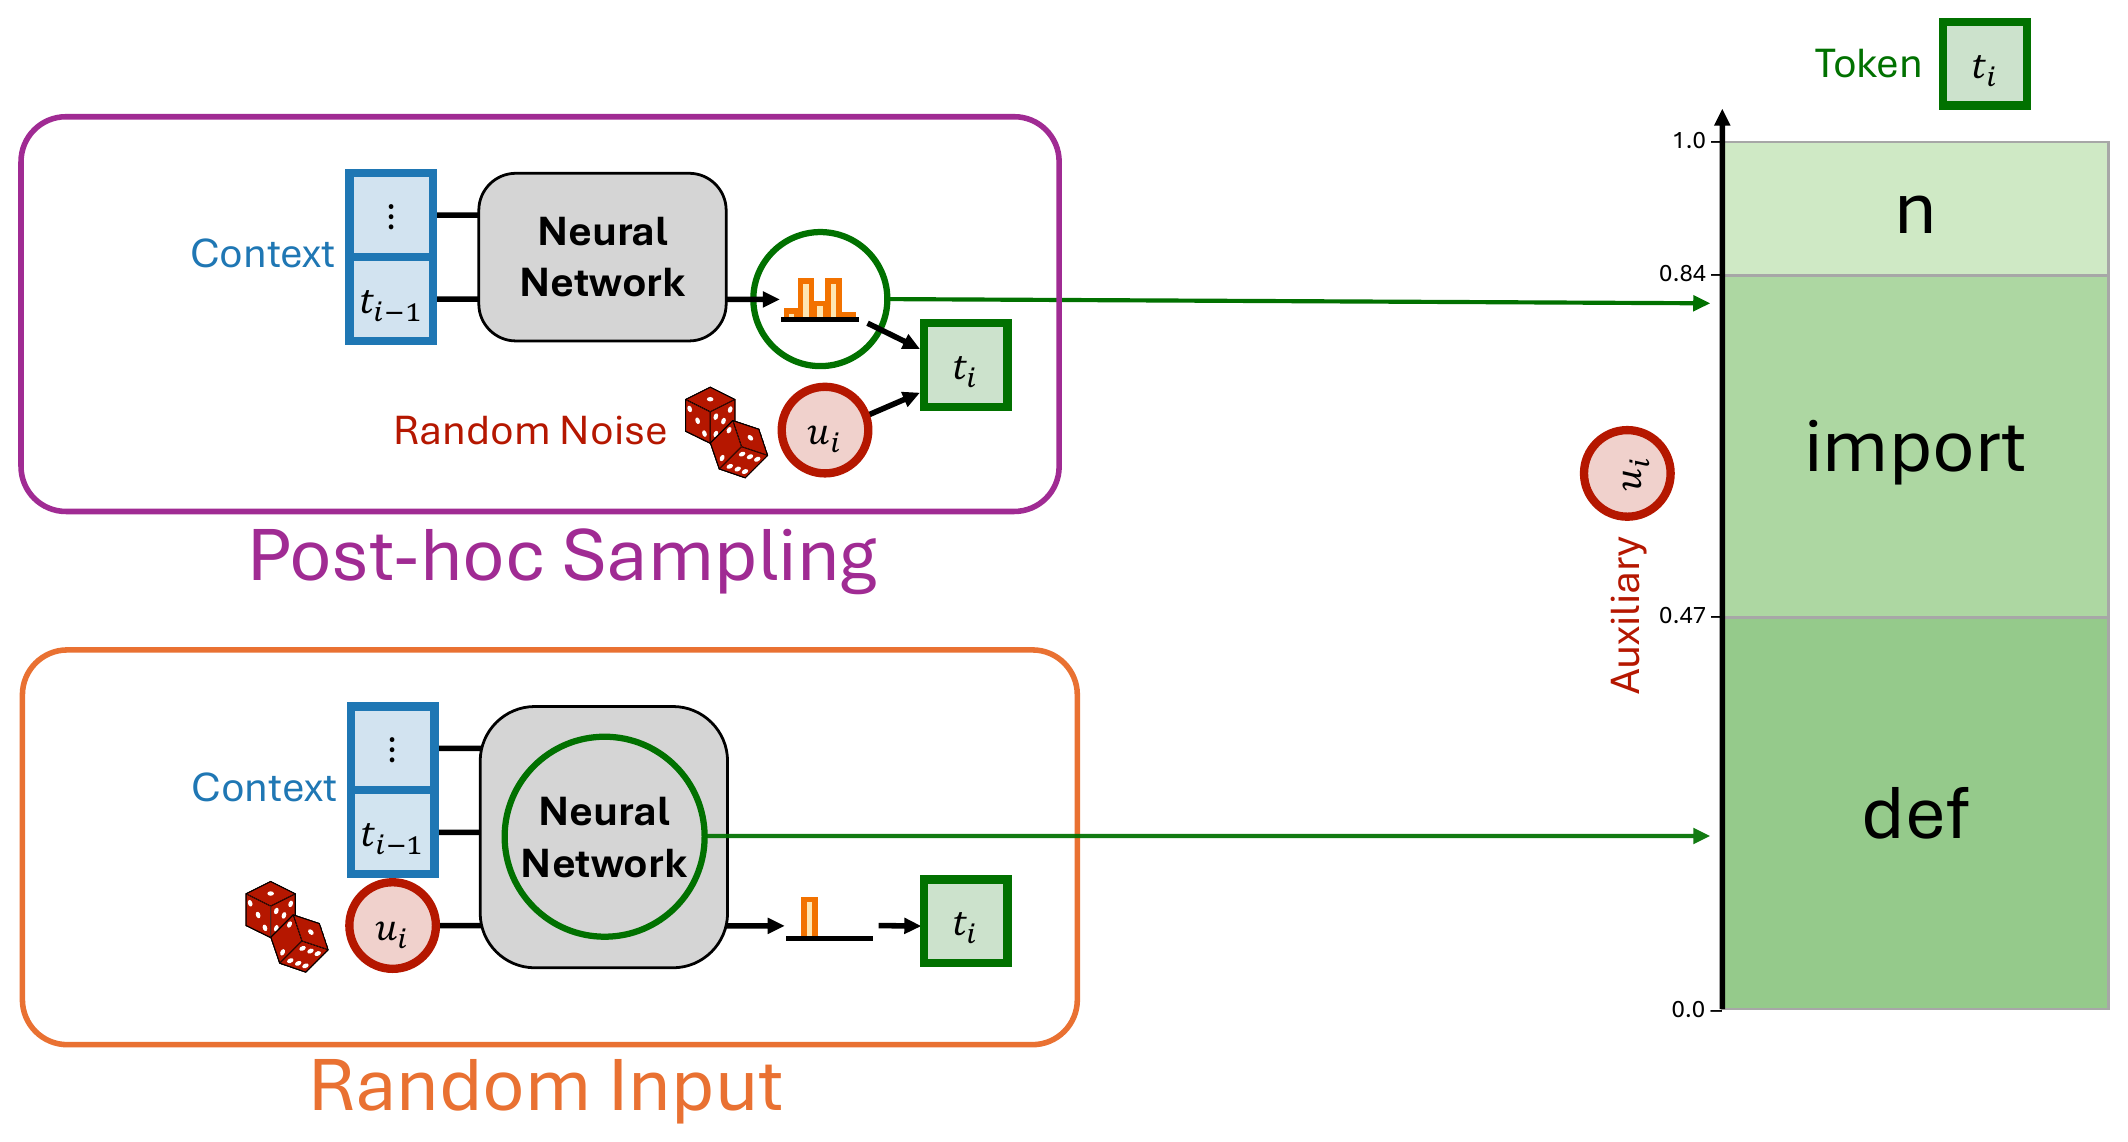
\includegraphics[width=0.78\textwidth]{ptp_auxiliaries.png}
  \caption{Moving the randomness. \textbf{Top:} standard decoding draws a
  distribution, then samples from it with auxiliary $\aux_i$. \textbf{Bottom:}
  PTP feeds $\aux_i$ in as an input, so the token becomes a deterministic
  function of context and auxiliaries and future tokens become jointly
  predictable. \textbf{Right:} $\aux_i$ selects a token by inverse CDF.
  Reproduced from the PTP framework~\citep{draxler2025ptp}.}
  \label{fig:auxiliaries}
\end{figure}

\subsection{What counts as a correct token}
\label{sec:correct}

Sharing the auxiliary variables gives verification a strong coupling. A proposed
token $t_k$ is \emph{correct} if it equals
$\tilde t_k = \Pick(\aux_k, \base(\cdot \mid t_{<k}))$, the token the base model
selects when the \emph{same} auxiliary is applied to its own distribution. Let
\begin{equation}
  \ncorrect = \max\{ m \geq 0 : t_{i+j} = \tilde t_{i+j} \text{ for all } j < m \}
\end{equation}
be the longest correct prefix. Because the base model evaluates
$\base(\cdot \mid t_{<k})$ at every position during verification anyway, one
token can be sampled from it for free at the first rejection, so a call commits
\begin{equation}
  \naccepted = \ncorrect + 1
  \label{eq:accepted}
\end{equation}
tokens. Under this rule the committed text is distributed exactly as the base
model's, so speedup is free of quality cost; the only question is how large
$\ncorrect$ is.

Figure~\ref{fig:partition} makes the geometry concrete for two tokens. The
auxiliary pair $(\aux_1, \aux_2)$ ranges over the unit square, and the AR
reference partitions that square into regions, one per token pair. A multi-token
model induces its own partition; where the two agree, the proposal is correct.
PTP's partition follows the reference's curved cell boundaries closely, whereas
independent per-position prediction can only produce a product partition of
axis-aligned rectangles and therefore mismatches over a large area.

\begin{figure}[t]
  \centering
  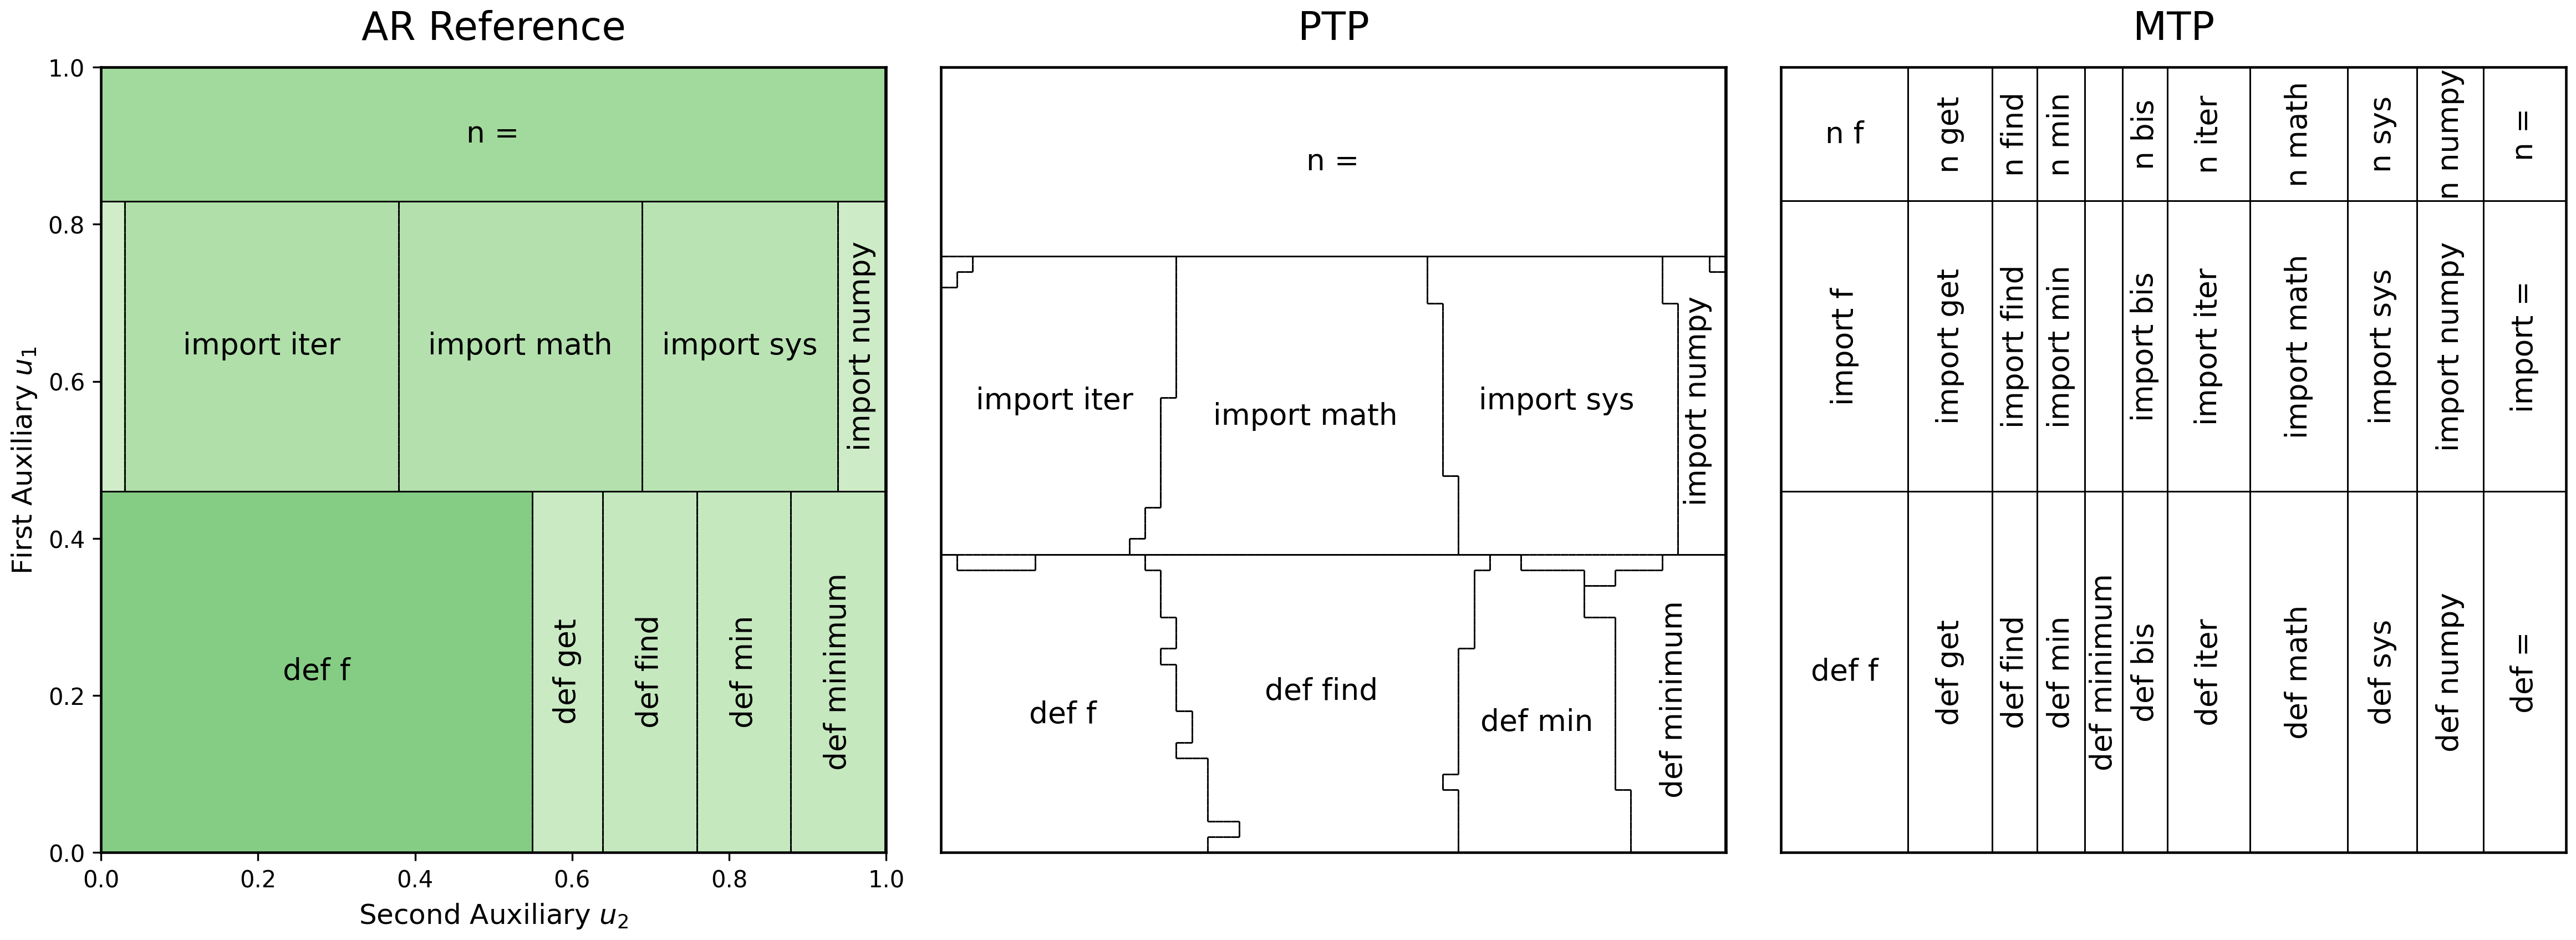
\includegraphics[width=\textwidth]{accept_partition.png}
  \caption{Verification as a partition-matching problem, for the first two
  generated tokens. The AR reference (left) partitions the auxiliary square into
  one cell per token pair. PTP (middle) reproduces the curved cell boundaries;
  independent multi-token prediction (right) can only form a product partition of
  rectangles. Correctness of a proposal is agreement of the two partitions at the
  drawn $(\aux_1, \aux_2)$. Reproduced from~\citet{draxler2025ptp}.}
  \label{fig:partition}
\end{figure}

\section{The acceptance layer}
\label{sec:acceptance}

\subsection{Exact acceptance is strict}

The rule of \S\ref{sec:correct} is exact but unforgiving: a proposal is rejected
whenever the drawn auxiliary falls in the sliver where the two partitions
disagree, even if the proposed token is one the base model would have been
perfectly happy to emit at a slightly different $\aux$. On the example of
Figure~\ref{fig:accept}, exact acceptance keeps $63\%$ of the auxiliary square;
relaxing the criterion to nucleus membership keeps $99\%$ of it, with the same
proposal model and the same proposals.

\begin{figure}[t]
  \centering
  \begin{subfigure}{\textwidth}
    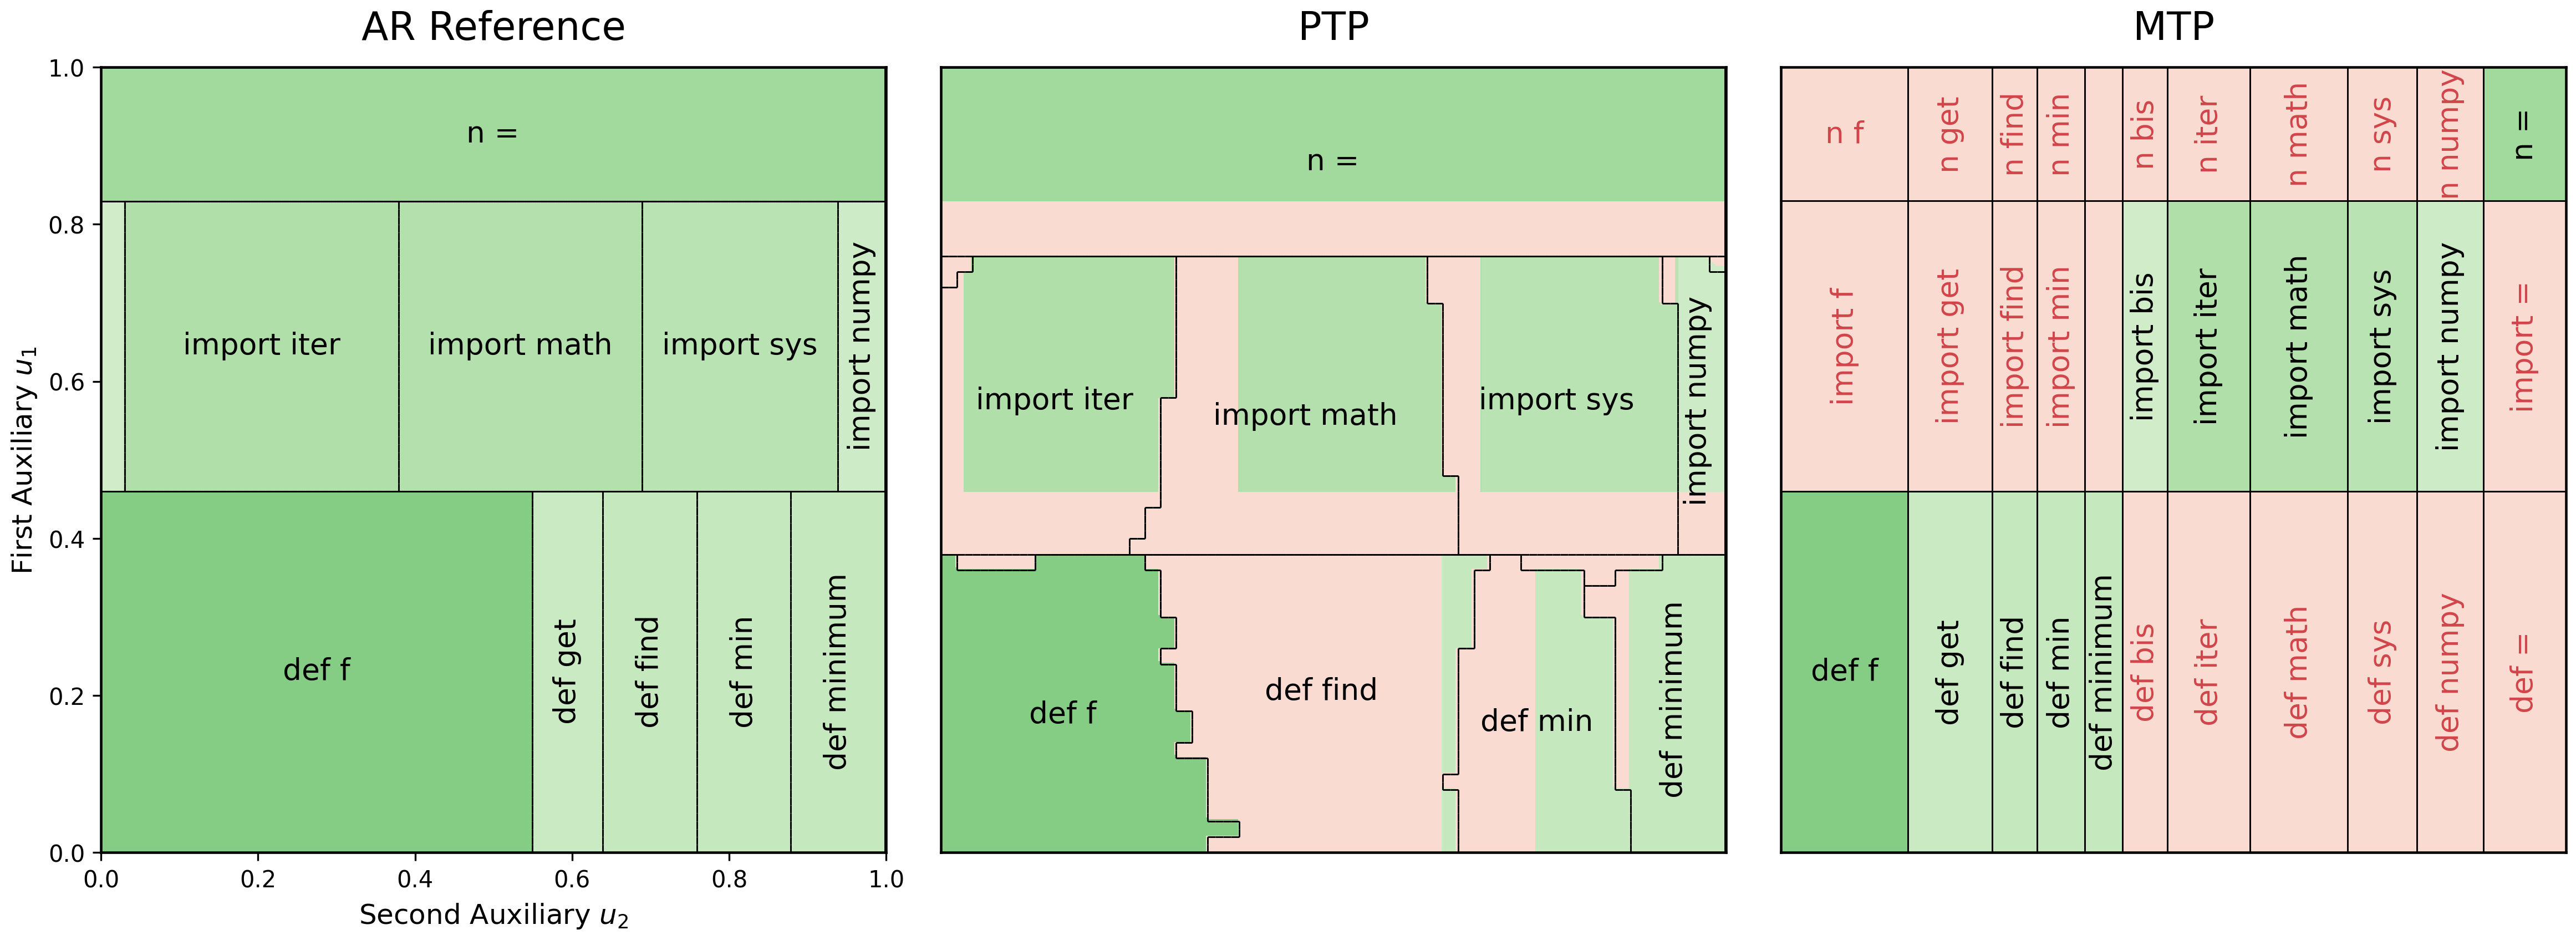
\includegraphics[width=\textwidth]{accept_exact.png}
    \caption{Exact acceptance: keep the proposal only where it \emph{equals} the
    reference token at the same auxiliary.}
  \end{subfigure}
  \\[0.6em]
  \begin{subfigure}{\textwidth}
    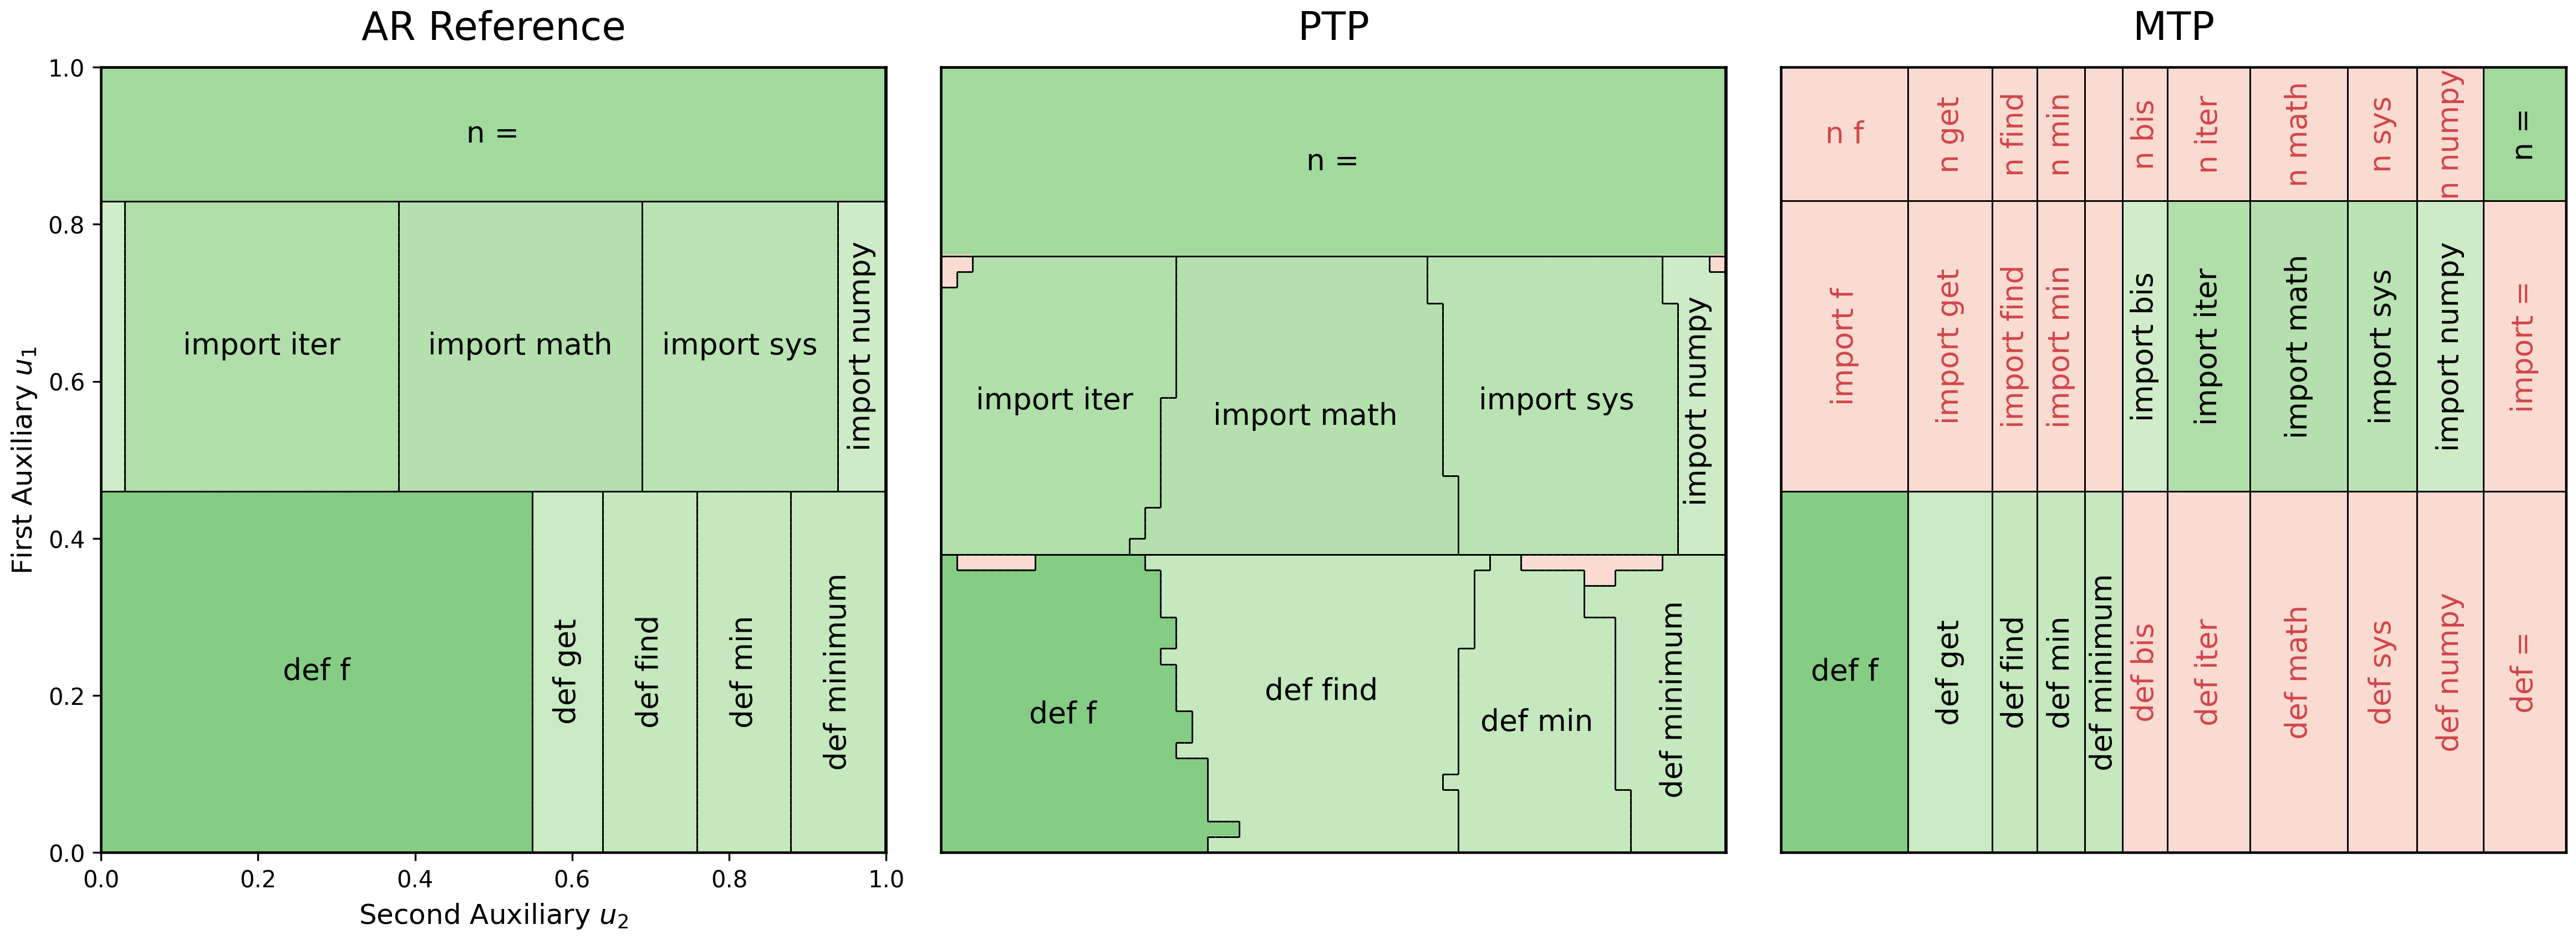
\includegraphics[width=\textwidth]{accept_nucleus.png}
    \caption{Broadened acceptance: keep the proposal wherever the reference finds
    the token plausible (nucleus membership).}
  \end{subfigure}
  \caption{The acceptance rule, not the model, decides what is kept. Both rows
  show the \emph{same} proposal partitions as Figure~\ref{fig:partition}; green
  is accepted, pink rejected. Broadening the criterion converts most of the
  rejected area into accepted area. This is the single largest lever in the
  design space, and the one that trades faithfulness for throughput most
  directly.}
  \label{fig:accept}
\end{figure}

\subsection{A taxonomy of rules}

Write $q$ for the proposal model's distribution at a position, $p$ for the base
model's, $x$ for the proposed token, and $\aux$ for the shared auxiliary. Every
rule we study decides acceptance from these objects; the families differ in what
they look at. All are implemented in a single code path so that the only
difference between two runs is the predicate.

\textbf{Exact.} Accept iff $x = \Pick(\aux, p)$. Distribution-preserving by
construction (\S\ref{sec:correct}).

\textbf{Relaxed deterministic.} Accept iff $x$ lies in a high-probability set of
$p$: nucleus membership, $\sum_{y : p(y) > p(x)} p(y) < \theta$
\citep{holtzman2020nucleus}, or top-$k$ rank. As $\theta \to 0$ this contracts to
argmax agreement, not to the exact rule.

\textbf{Thresholds.} Accept iff $p(x) \geq \theta$ (base-model probability), or
iff $q(x) \geq \theta$ (the proposal model's own confidence). The latter needs no
base-model call at all, which makes it the cheapest rule available and, as we
show, not a good one.

\textbf{Stochastic ratio.} The speculative-sampling
rule~\citep{leviathan2023speculative,chen2023accelerating}: accept with
probability $\min(1, (\kappa \, p(x) + \varpi)/q(x))$ and, on rejection, resample
from the residual $\propto \max(0, p - q)$. At $\kappa = 1, \varpi = 0$ this is
distribution-preserving in theory.

\textbf{Inverse-CDF distance.} Accept iff the drawn $\aux$ is within $\theta$ of
the interval $[\aux_{\mathrm{lo}}, \aux_{\mathrm{hi}})$ that $p$ assigns to $x$,
\ie $\max(\aux_{\mathrm{lo}} - \aux,\, \aux - \aux_{\mathrm{hi}}) \leq \theta$.
This interpolates continuously from the exact rule at $\theta = 0$, and is the
natural relaxation in the auxiliary-square picture of
Figure~\ref{fig:accept}: it dilates the accepted cell rather than replacing the
criterion.

\textbf{Unconditional.} Accept the first $k$ proposed tokens regardless. A
throughput ceiling and a quality floor.

\textbf{Self-verification.} Replace the base model by the proposal model's own
autoregressive prediction, so no second set of weights is consulted. This removes
the base-model call from the critical path entirely; the cost is that the rule no
longer references the distribution we are trying to stay faithful to.

Only the exact rule and (in theory) the ratio rule preserve the base model's
output distribution. Every other rule biases the output, and the empirical
question is by how much, in exchange for what.

\section{A model of the number of correct tokens}
\label{sec:model}

The verification axis fixes \emph{when} a token is kept. The geometry axis asks
how many proposals to make and how long each should be, and answering it requires
knowing how $\ncorrect$ behaves. We therefore assume a model of $\ncorrect$ given
the number of proposal strands $K$ and the context, and we will need from it only
the survival function
\begin{equation}
  \Sfun[w, d] \;=\; \Pr\big[\, \extinct \geq d \,\big|\, w \text{ strands} \,\big],
  \qquad \extinct = \naccepted - 1,
  \label{eq:survival}
\end{equation}
where $\extinct$ is the number of generations before every strand has failed
verification and, following \eqref{eq:accepted}, $G := \naccepted = 1 + \extinct$
is the committed token count per call.

\subsection{Geometric and beta-geometric baselines}

The simplest model treats each accepted token as an independent coin flip with
success probability $p$, making $\extinct$ geometric:
\begin{equation}
  \Sfun[1, d] = p^{\,d-1},
  \qquad \Pr[\extinct = d] = (1-p)\,p^{\,d-1}.
  \label{eq:geometric}
\end{equation}
For a single strand this is already a good description:
Figure~\ref{fig:geometric} fits \eqref{eq:geometric} to $5{,}070$ observed calls
at $K=1$ with $R^2 = 0.999$. Allowing the acceptance probability to vary across
prompts, $p \sim \mathrm{Beta}(a, b)$, gives the beta-geometric model
\begin{equation}
  \Pr[\extinct = d] = \int_0^1 (1-p)\,p^{\,d-1}\,\mathrm{Beta}(p; a, b)\,\mathrm{d}p
  = \frac{B(a + d - 1,\, b + 1)}{B(a, b)},
  \label{eq:betageom}
\end{equation}
which matters because that variation is real: a likelihood-ratio test against a
single pooled $p$ rejects homogeneity decisively
($\chi^2 = 401$ on $99$ degrees of freedom, $p \approx 5 \times 10^{-38}$;
Figure~\ref{fig:heterogeneity}).

\begin{figure}[t]
  \centering
  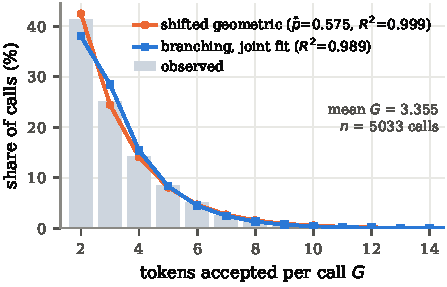
\includegraphics[width=0.62\textwidth]{geometric.pdf}
  \caption{Committed tokens per call at $K=1$. A shifted geometric
  \eqref{eq:geometric} fitted to this width alone is already excellent; the
  branching model of \S\ref{sec:branching}, fitted \emph{jointly} across all five
  widths, gives up a little accuracy here in exchange for extrapolating across
  $K$ (Figure~\ref{fig:vsk}). Preliminary single-seed run.}
  \label{fig:geometric}
\end{figure}

\subsection{Ensembles need a correlated model}
\label{sec:branching}

Neither baseline survives the move to $K > 1$ strands. If strands failed
independently, total wipeout would vanish geometrically in $K$; empirically
$\Pr[\extinct = 1]$ falls from $41\%$ at $K = 1$ only to $13\%$ at $K = 1000$ and
flattens against a floor (Figure~\ref{fig:vsk}, left). Some positions are simply
hard, and no ensemble width rescues them.

We therefore model the strands as a branching process with a frailty that is
\emph{shared} within each generation. At depth $i$, given $\alive_{i-1} = m$
surviving strands,
\begin{equation}
  \frail_i \sim \pizero \, \delta_0 + (1 - \pizero)\,\mathrm{Beta}(\alpha, \beta),
  \qquad
  \alive_i \mid \alive_{i-1} = m,\, \frail_i \;\sim\; \mathrm{Binomial}(m, \frail_i),
  \label{eq:branching}
\end{equation}
with $\extinct = \min\{i \geq 1 : \alive_i = 0\}$. We parameterize by the
marginal per-strand success probability $p$ and the within-generation correlation
$\rhoc$ between two strands,
\begin{equation}
  \nu = \frac{1 - \rhoc}{\rhoc}, \qquad \alpha = p\,\nu, \qquad \beta = (1-p)\,\nu .
  \label{eq:reparam}
\end{equation}
Two features are load-bearing. The shared draw of $\frail_i$ correlates strands
within a generation: they tend to fail together, which is why width has
diminishing returns. The point mass $\pizero$ at $\frail = 0$ makes a fraction of
positions a guaranteed wipeout regardless of $K$, producing the observed floor;
a pure Beta-Binomial cannot. Marginalizing $\frail_i$ gives a Beta-Binomial
transition kernel
\begin{equation}
  P[m, j] = (1 - \pizero)\,\BetaBin(j \mid m, \alpha, \beta) + \pizero \, \mathbb{1}[j = 0],
  \label{eq:kernel}
\end{equation}
with $0$ absorbing, from which $\Sfun[w, \cdot]$ follows by propagation. Following
the structure of the decoder, generation $1$ is exempt from zero-inflation and
the terminal generation $\capt$ is a forced death, reflecting the hard
proposal-length cap. Fitting $(\pizero, p, \rhoc)$ by joint maximum likelihood
over all five widths simultaneously gives
$\pizero = 0.128$, $p = 0.620$, $\rhoc = 0.789$ on our checkpoint.

\begin{figure}[t]
  \centering
  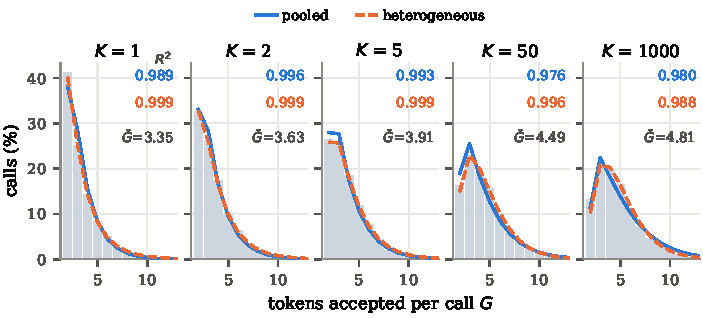
\includegraphics[width=\textwidth]{hist_by_k.pdf}
  \caption{Committed tokens per call against ensemble width. Bars are observed;
  lines are the branching model \eqref{eq:branching} with a single
  $(\pizero, p, \rhoc)$ shared across all five panels (\emph{pooled}) and with
  $p$ integrated over a fitted $\mathrm{Beta}(a,b)$ population
  (\emph{heterogeneous}). $R^2$ per curve is printed in the curve's own colour.
  One three-parameter model tracks the distribution over three orders of
  magnitude of $K$.}
  \label{fig:histbyk}
\end{figure}

\begin{figure}[t]
  \centering
  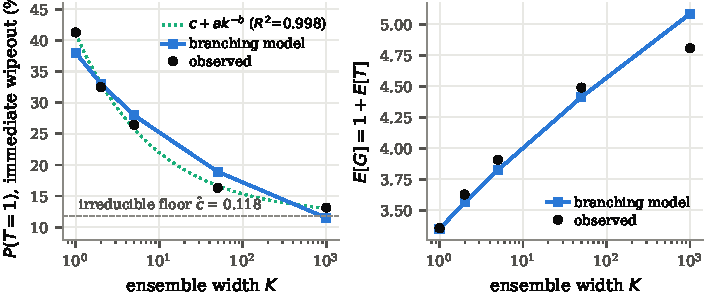
\includegraphics[width=\textwidth]{vs_k.pdf}
  \caption{Why width saturates. \textbf{Left:} the probability of immediate
  wipeout decays towards an irreducible floor $\hat c = 0.118$, not to zero; a
  phenomenological $c + a K^{-b}$ captures this, and the branching model produces
  it from $\pizero$. \textbf{Right:} committed tokens per call grow roughly
  logarithmically in $K$ --- a $1000\times$ increase in proposal width buys about
  $1.5$ extra tokens.}
  \label{fig:vsk}
\end{figure}

\section{From survival to allocation: the strand-length knapsack}
\label{sec:knapsack}

Strands need not all be the same length. Let $L_s$ be the length budgeted to
strand $s$ and define the \emph{width profile}
\begin{equation}
  \width(d) := \#\{ s : L_s \geq d \},
  \label{eq:widthprofile}
\end{equation}
the number of strands still budgeted to reach depth $d$. The key structural fact
is that the shared frailty $\frail_d$ acts conditionally i.i.d.\ on every strand
present in generation $d$, so any fixed subset of a surviving population is
itself Beta-Binomial with the same $(\alpha, \beta)$ --- a thinning property.
Consequently the subpopulation that is both alive and still within its own budget
at depth $d$ is distributed exactly as a fresh homogeneous run started with
$\width(d)$ strands, \emph{independently of every other depth}, and the tail-sum
identity gives
\begin{equation}
  \mathbb{E}[\extinct] \;=\; \sum_{d \geq 1} \Pr[\extinct \geq d] \;=\; \sum_{d=1}^{\capt} \Sfun[\width(d), d].
  \label{eq:separable}
\end{equation}
Expected yield is a sum of terms each depending on the width profile at a
\emph{single} depth. That separability is what makes the design problem tractable.

Choosing strand lengths under a node budget is then
\begin{equation}
  \max_{L_1, \dots, L_K} \; \sum_{d=1}^{\capt} \Sfun[\width(d), d]
  \qquad \text{s.t.} \qquad \sum_{s} L_s \leq \budget ,
  \label{eq:knapsack}
\end{equation}
a knapsack whose items are \emph{whole strands}: buying a strand of length $L$
raises the width at every depth $1, \dots, L$ at once, so its cost is $L$ and its
value is the bundled gain across those depths.

\paragraph{Exact solution.}
The feasible width profiles are exactly the nonincreasing integer sequences
$\width(1) \geq \dots \geq \width(\capt) \geq 0$: any such sequence decomposes
into $\width(d) - \width(d+1)$ strands of length $d$, by the standard
correspondence between nonincreasing sequences and partitions, and its cost
$\sum_d \width(d)$ equals the sum of those lengths. So \eqref{eq:knapsack} is a
maximization over nonincreasing profiles, solved exactly by a dynamic program
over depth:
\begin{equation}
  V_d[w_{\mathrm{cap}}, b] \;=\; \max_{0 \leq w \leq \min(w_{\mathrm{cap}},\, b)}
  \Big\{ \Sfun[w, d] + V_{d+1}[w,\, b - w] \Big\},
  \qquad V_{\capt + 1} \equiv 0,
  \label{eq:dp}
\end{equation}
where $V_d[w_{\mathrm{cap}}, b]$ is the best achievable
$\sum_{d' \geq d} \Sfun[\width(d'), d']$ given $\width(d) \leq w_{\mathrm{cap}}$
and remaining budget $b$. Doubling the width bound until the optimum stops
touching it makes the result exact at any budget.

\begin{figure}[t]
  \centering
  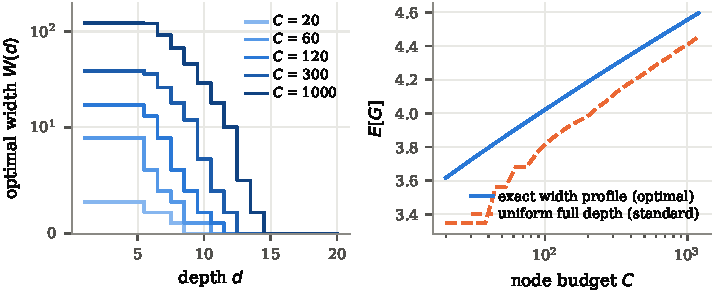
\includegraphics[width=\textwidth]{width_profile.pdf}
  \caption{The allocation solved by \eqref{eq:dp}. \textbf{Left:} optimal width
  profiles at several node budgets --- wide and shallow, never uniform.
  \textbf{Right:} what the exact profile buys over spending the same budget on
  full-depth strands (the \texttt{standard} allocation). The gap is roughly
  $0.15$--$0.2$ committed tokens per call across two decades of budget.}
  \label{fig:widthprofile}
\end{figure}

\subsection{Combining with Partial Quadratic Decoding}
\label{sec:pqd}

Speculative decoding runs proposal and verification in sequence. PQD removes that
serialization by speculating on the verification outcome: while the base model
verifies $\nprop$ proposed tokens, the proposal model prepares a branch for each
possible $m \in \{0, \dots, \nprop\}$, each conditioned on ``exactly $m$ of the
proposed tokens were correct'' (Figure~\ref{fig:pqd}). When verification returns
$m^\ast$, the other branches are discarded and generation continues from the
precomputed branch $m^\ast$.

\begin{figure}[t]
  \centering
  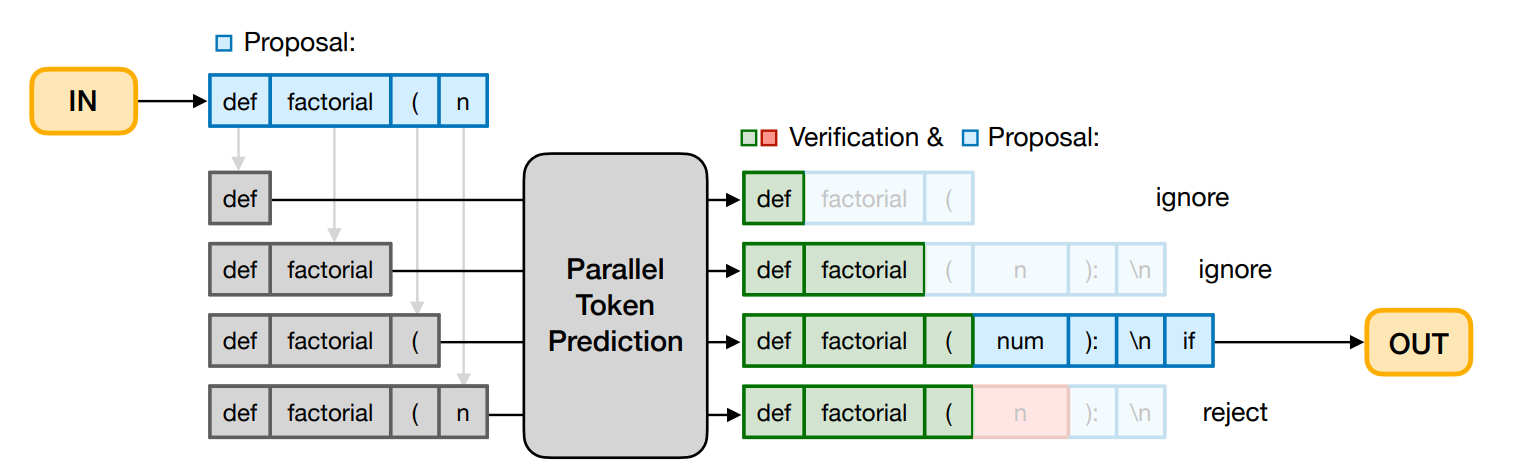
\includegraphics[width=0.92\textwidth]{pqd_branches.png}
  \caption{Partial Quadratic Decoding. One branch is prepared per possible number
  of correct tokens, concurrently with verification; when the base model returns
  $m^\ast$, the matching branch is already extended and the rest are discarded.
  Reproduced from~\citet{draxler2025ptp}.}
  \label{fig:pqd}
\end{figure}

PQD must decide how many continuation tokens $B_m$ to give each branch under a
total budget $\budget$, which it does by maximizing an expected utility
\begin{equation}
  \max_{\sum_m B_m = \budget} \; \sum_{m} \Pr[\ncorrect = m \mid t] \; H(B_m),
  \label{eq:pqd}
\end{equation}
solved greedily by marginal gain. As originally formulated, the two ingredients
of \eqref{eq:pqd} come from different places: the branch weights are estimated by
treating errors as independent given the proposal model's confidences,
$\Pr[\ncorrect = m \mid t] \approx (1 - c_{i+m}) \prod_{k < i+m} c_k$, while the
reward $H$ is a separate monotone function calibrated on the training set.

\S\ref{sec:model} supplies both from one object. The branch weights are the
increments of the survival function,
\begin{equation}
  \Pr[\ncorrect = m] \;=\; \Sfun[K, m] - \Sfun[K, m+1],
  \label{eq:branchweights}
\end{equation}
and the value of giving a branch $n$ tokens is the expected yield of the optimal
allocation of those $n$ tokens, \ie the dynamic program \eqref{eq:dp}:
\begin{equation}
  H(n) \;=\; \max_{\width \text{ nonincreasing},\; \sum_d \width(d) \leq n} \; \sum_{d} \Sfun[\width(d), d] \;=\; V_1[\infty, n].
  \label{eq:H}
\end{equation}
Both ingredients are then consistent by construction, calibrated by the same
three parameters, and --- because $H$ is the \emph{optimal} yield rather than a
heuristic proxy --- the greedy allocation in \eqref{eq:pqd} is comparing branches
on the quantity it actually cares about. The independence approximation is
retained only where per-position confidences are genuinely more informative than
the pooled model, namely in conditioning $\Sfun$ on context; \S\ref{sec:exp:ens}
compares pooled, Bayesian-updated, and learned-head estimates of $p$ empirically.

\subsection{Worked example}
\label{sec:worked}

Table~\ref{tab:survival} gives the fitted survival function at our checkpoint's
$(\pizero, p, \rhoc) = (0.128, 0.620, 0.789)$. Two things stand out.
$\Sfun[w, 1] = 1$ for every $w \geq 1$, so width has \emph{zero} marginal value at
depth $1$ --- a single strand always reaches the first generation. And the
returns to width at a fixed depth are strongly concave: at depth $4$, going from
$1$ to $2$ strands buys more than going from $5$ to $50$.

Table~\ref{tab:knapsack} turns this into allocations. At a budget of
$\budget = 1000$ nodes --- the setting our $K = 50$ runs use --- the optimum is
$122$ strands of mixed length, from $2$ of depth $14$ down to $29$ of depth $6$,
and it yields $4.555$ committed tokens per call against $4.412$ for $50$ strands
at full depth $20$. The exact solver reallocates the deep tail of the uniform
profile into extra width at shallow depths, where the survival table says it is
worth more.

\begin{table}[t]
  \centering
  \caption{Fitted survival function $\Sfun[w, d] = \Pr[\extinct \geq d]$ for a
  homogeneous run of $w$ strands, at $(\pizero, p, \rhoc) = (0.128, 0.620,
  0.789)$. Width has no value at depth $1$ and sharply diminishing value
  thereafter.}
  \label{tab:survival}
  \begin{tabular}{rrrrrrrr}
\toprule
& \multicolumn{7}{c}{depth $d$} \\
\cmidrule(lr){2-8}
$w$ & 1 & 2 & 3 & 4 & 5 & 6 & 8 \\
\midrule
1 & 1.000 & 0.620 & 0.335 & 0.181 & 0.098 & 0.053 & 0.015 \\
2 & 1.000 & 0.670 & 0.386 & 0.221 & 0.125 & 0.071 & 0.022 \\
5 & 1.000 & 0.720 & 0.444 & 0.269 & 0.161 & 0.096 & 0.033 \\
50 & 1.000 & 0.811 & 0.557 & 0.373 & 0.245 & 0.159 & 0.064 \\
\bottomrule
\end{tabular}
\end{table}

\begin{table}[t]
  \centering
  \caption{Optimal versus uniform allocation of a node budget, under the fitted
  model. The profile column reads $\mathrm{depth}^{\mathrm{count}}$, so
  $6^{29}$ means $29$ strands of length $6$. The exact profile trades depth for
  width and gains $\approx 0.15$ committed tokens per call.}
  \label{tab:knapsack}
  {\setlength{\tabcolsep}{4pt}%
\begin{tabular}{rllrr}
\toprule
\multicolumn{1}{c}{budget $\budget$} & allocation & \multicolumn{1}{c}{profile $\mathrm{depth}^{\mathrm{count}}$} & \multicolumn{1}{c}{strands} & \multicolumn{1}{c}{$E[G]$} \\
\midrule
120 & exact profile & $11^{1}\,10^{1}\,9^{2}\,8^{2}\,7^{3}\,6^{4}\,5^{4}$ & 17 & 4.067 \\
 & uniform full depth & $20^{6}$ & 6 & 3.873 \\
300 & exact profile & $12^{2}\,11^{2}\,10^{3}\,9^{5}\,8^{6}\,7^{8}\,6^{10}\,5^{3}$ & 39 & 4.282 \\
 & uniform full depth & $20^{15}$ & 15 & 4.114 \\
1000 & exact profile & $14^{2}\,13^{3}\,12^{5}\,11^{8}\,10^{11}\,9^{17}\,8^{21}\,7^{25}\,6^{29}\,5^{1}$ & 122 & 4.555 \\
 & uniform full depth & $20^{50}$ & 50 & 4.412 \\
\bottomrule
\end{tabular}
}
\end{table}

\section{Experiments}
\label{sec:experiments}

\subsection{Setup}

We distil a one-hot PTP student from Vicuna-7B-v1.5~\citep{zheng2023vicuna} with
gated LoRA adapters~\citep{hu2022lora} of rank $128$ and a binary auxiliary
embedding, and evaluate on the first turns of the $13$ Spec-Bench
categories~\citep{xia2024specbench} ($100$ questions), with temperature $0.7$,
top-$k$ $50$, top-$p$ $0.9$, at most $20$ proposed tokens per strand and a total
budget of $120$ proposed tokens per call, on a single NVIDIA RTX A6000.

We report three families of measure, deliberately kept separate.
\emph{Throughput per call} is $\naccepted$ averaged over calls.
\emph{Wall-clock} is milliseconds per generated token, and speedup is the AR
run's ms/token divided by the rule's --- so it charges every rule for the compute
it actually spends. \emph{Faithfulness} is measured under the base model:
$\bar q$ is the mean per-token probability the base model assigns to the
generated tokens ($\%$), PPL the corresponding perplexity, and
$p_{\mathrm{align}}$ the $p$-value of a pooled CLT $z$-test of the null
hypothesis that the generated tokens were drawn from the base distribution. A
large $p_{\mathrm{align}}$ is the operational meaning of ``indistinguishable from
the base model''.

\subsection{Acceptance rules: three orderings, not one}
\label{sec:exp:rules}

Table~\ref{tab:rules} is the main result. The headline is that the three measures
disagree.

\begin{table}[t]
  \centering
  \caption{Acceptance rules on Spec-Bench. $\bar q$ is the mean per-token
  probability under the base model, $p_{\mathrm{align}}$ the $p$-value for
  ``generated tokens came from the base distribution''. $^\dagger$
  distribution-preserving by construction. Numbers are preliminary: single-seed
  runs on $100$ Spec-Bench first turns.}
  \label{tab:rules}
  \small
  {\setlength{\tabcolsep}{4pt}%
\begin{tabular}{llrrrrrr}
\toprule
acceptance rule & setting & \multicolumn{1}{c}{tok./call} & \multicolumn{1}{c}{ms/tok.} & \multicolumn{1}{c}{speedup} & \multicolumn{1}{c}{$\bar q$ (\%)} & \multicolumn{1}{c}{PPL} & \multicolumn{1}{c}{$p_{\mathrm{align}}$} \\
\midrule
autoregressive$^\dagger$ & -- & 1.00 & 56.4 & 1.00$\times$ & 84.15 & 1.20 & 0.251 \\
PTP, single call$^\dagger$ & -- & 2.39 & 32.7 & 1.73$\times$ & 84.51 & 1.19 & 0.247 \\
PTP, sequential$^\dagger$ & -- & 3.63 & 55.3 & 1.02$\times$ & 84.71 & 1.19 & 0.799 \\
nucleus & $\theta=0.9$ & 3.88 & 35.4 & 1.59$\times$ & 74.09 & 1.40 & $<$0.001 \\
nucleus & $\theta=0.98$ & 4.30 & 33.2 & 1.70$\times$ & 67.58 & 1.56 & $<$0.001 \\
nucleus + ensemble & $\theta=0.98$, $K=5$ & 4.32 & 57.4 & 0.98$\times$ & 82.92 & 1.22 & $<$0.001 \\
nucleus + ensemble & $\theta=0.98$, $K=50$ & 4.74 & 140.4 & 0.40$\times$ & 82.97 & 1.22 & $<$0.001 \\
speculative ratio & -- & 2.35 & 34.3 & 1.65$\times$ & 69.94 & 1.58 & $<$0.001 \\
speculative ratio & $\kappa=10$ & 2.62 & 31.0 & 1.82$\times$ & 70.12 & 1.57 & $<$0.001 \\
teacher threshold & $\theta=0.1$ & 3.58 & 46.0 & 1.23$\times$ & 83.16 & 1.21 & $<$0.001 \\
teacher threshold & $\theta=0.5$ & 3.22 & 52.3 & 1.08$\times$ & 85.26 & 1.18 & $<$0.001 \\
student confidence & $\theta=0.5$ & 2.01 & 69.4 & 0.81$\times$ & 41.42 & 17.03 & $<$0.001 \\
student confidence & $\theta=0.9$ & 1.34 & 92.7 & 0.61$\times$ & 64.95 & 1.77 & 0.006 \\
accept-$k$ & $k=2$ & 2.00 & 31.7 & 1.78$\times$ & 49.29 & 40.92 & $<$0.001 \\
accept-$k$ & $k=4$ & 4.00 & 16.1 & 3.50$\times$ & 47.34 & 31.99 & $<$0.001 \\
self-verified & exact & 3.86 & 49.9 & 1.13$\times$ & 65.92 & 1.60 & $<$0.001 \\
self-verified + nucleus & $\theta=0.8$ & 6.45 & 39.8 & 1.42$\times$ & 24.66 & 38.70 & $<$0.001 \\
self-verified + ensemble & $\theta=0.8$, $K=50$ & 5.98 & 111.1 & 0.51$\times$ & 73.74 & 1.40 & $<$0.001 \\
\bottomrule
\end{tabular}
}
\end{table}

\textbf{Tokens per call is not speed.} Sequential exact PTP commits $3.63$ tokens
per call --- more than any single-call rule --- yet reaches only $1.02\times$,
because its proposal and verification passes are serialized. The single-call
variant commits $2.39$ and reaches $1.73\times$. Ensembles push tokens per call
to $4.74$ and wall-clock \emph{down} to $0.40\times$: at $K = 50$ the $1000$
proposal nodes cost more than the tokens they save. This is precisely the regime
PQD (\S\ref{sec:pqd}) exists to fix, and it is invisible if one reports only
accepted-tokens-per-call.

\textbf{Only the exact rules are faithful.} The $z$-test separates the two
classes cleanly: $p_{\mathrm{align}} = 0.25$ and $0.80$ for exact PTP, versus
$< 0.001$ for every relaxed rule. Broadening to nucleus $\theta = 0.98$ costs
$16.6$ points of $\bar q$ ($84.5 \to 67.6$) to gain $1.9$ tokens per call.

\textbf{Cheap rules are bad rules.} Student-confidence thresholding needs no
base-model call, and is the worst rule in the table on every axis at once: at
$\theta = 0.5$ it commits $2.01$ tokens per call, runs \emph{slower} than AR
($0.81\times$), and collapses quality to $\mathrm{PPL} = 17.0$. Accepting $k$
tokens unconditionally is the honest version of the same trade: $3.50\times$ at
$k = 4$, with $\mathrm{PPL} = 32.0$.

\textbf{An anomaly worth flagging.} The stochastic ratio rule is
distribution-preserving in theory at $\kappa = 1, \varpi = 0$, but we measure
$\bar q = 69.9$ and $p_{\mathrm{align}} < 0.001$ --- a clear deviation. We have
not marked it as lossless in Table~\ref{tab:rules} for that reason. Resolving
whether this is an artefact of residual resampling in the truncated top-$k$ space
or a genuine implementation defect is left to future work; we report it rather
than assume the theory.

\begin{figure}[t]
  \centering
  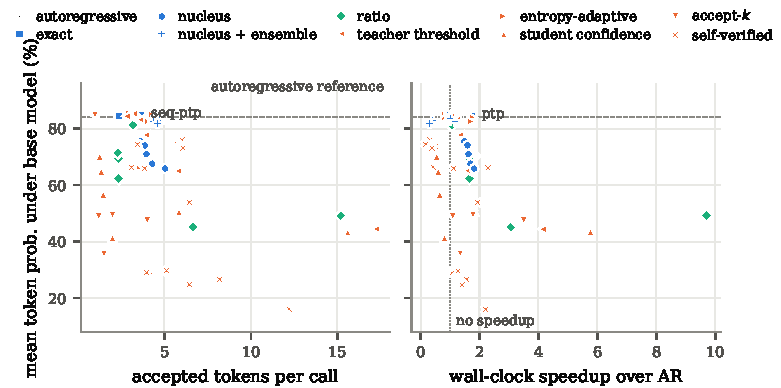
\includegraphics[width=\textwidth]{pareto.pdf}
  \caption{Throughput against faithfulness for all $62$ configurations. The two
  panels share a $y$-axis but order the rules differently: high tokens per call
  (left) does not imply wall-clock speedup (right). Only the exact rules sit on
  the autoregressive reference line.}
  \label{fig:pareto}
\end{figure}

\subsection{Threshold sweeps}

Figure~\ref{fig:sweeps} sweeps $\theta$ for the three threshold-style families.
Base-model-probability thresholding degrades gracefully and monotonically: as
$\theta \to 0$ it accepts everything, reaching $17$ tokens per call and
$4.1\times$, and as $\theta$ grows it recovers the base model's quality. Nucleus
acceptance occupies a narrow, useful band near $\theta \approx 0.9$--$0.98$.
Student-confidence thresholding is non-monotone and dominated everywhere.

\begin{figure}[t]
  \centering
  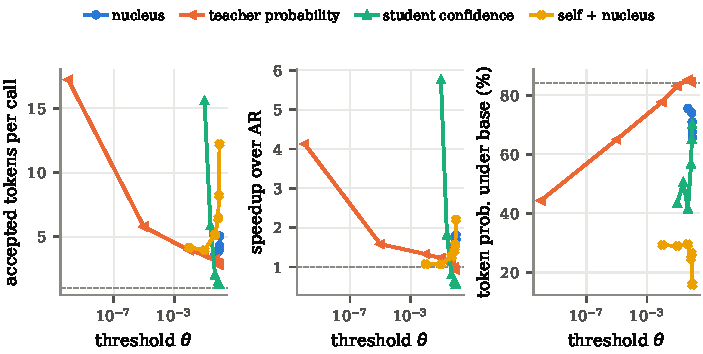
\includegraphics[width=\textwidth]{sweeps.pdf}
  \caption{Threshold sweeps. Separate panels rather than twin axes, because the
  three measures are on unrelated scales. Dashed lines mark the autoregressive
  reference.}
  \label{fig:sweeps}
\end{figure}

\subsection{Ensembles and allocation}
\label{sec:exp:ens}

Table~\ref{tab:ensemble} varies how the per-strand acceptance probability driving
the allocation of \S\ref{sec:knapsack} is estimated: a single pooled $p$, an
online Bayesian update (conjugate Beta-Binomial, or a grid reweighted by the
survival likelihood), and a small learned head predicting $p$ from the hidden
state. Differences are modest at $K = 5$ and grow at $K = 50$, consistent with
the allocation mattering more when there is more budget to misallocate.

\begin{table}[t]
  \centering
  \caption{Estimating the allocation's acceptance probability. All rows use the
  nucleus criterion at the stated $\theta$; ``allocation'' is how $p$ is
  estimated for the knapsack of \S\ref{sec:knapsack}. Preliminary.}
  \label{tab:ensemble}
  \small
  {\setlength{\tabcolsep}{4pt}%
\begin{tabular}{llrrrrr}
\toprule
verification & allocation & \multicolumn{1}{c}{$K$} & \multicolumn{1}{c}{tok./call} & \multicolumn{1}{c}{ms/tok.} & \multicolumn{1}{c}{speedup} & \multicolumn{1}{c}{$\bar q$ (\%)} \\
\midrule
verified against the base model, $\theta=0.98$ & uniform & 5 & 4.32 & 57.4 & 0.98$\times$ & 82.92 \\
 & Bayes, conjugate & 5 & 4.46 & 55.9 & 1.01$\times$ & 83.52 \\
 & Bayes, grid & 5 & 4.38 & 48.2 & 1.17$\times$ & 82.46 \\
 & uniform & 50 & 4.74 & 140.4 & 0.40$\times$ & 82.97 \\
 & Bayes, conjugate & 50 & 4.77 & 159.8 & 0.35$\times$ & 82.02 \\
 & Bayes, grid & 50 & 4.60 & 182.1 & 0.31$\times$ & 81.88 \\
\midrule
self-verified, $\theta=0.8$ & uniform & 50 & 5.98 & 111.1 & 0.51$\times$ & 73.74 \\
 & Bayes, conjugate & 50 & 6.03 & 179.0 & 0.32$\times$ & 76.04 \\
 & Bayes, grid & 50 & 5.77 & 201.8 & 0.28$\times$ & 74.29 \\
 & learned $p$-head & 50 & 3.45 & 325.4 & 0.17$\times$ & 74.48 \\
\bottomrule
\end{tabular}
}
\end{table}

\subsection{Does the model predict the data?}

Table~\ref{tab:fit} and Figure~\ref{fig:histbyk} validate \S\ref{sec:model}. One
three-parameter model, fitted jointly, reproduces the per-call histogram at every
width with $R^2 \in [0.976, 0.996]$ and predicts $\mathbb{E}[G]$ to within
$0.08$ tokens at $K \leq 50$. It degrades at $K = 1000$ (predicting $5.09$ against
an observed $4.81$), which is the extrapolation limit of a depth-uniform
$(\pizero, p, \rhoc)$. Integrating $p$ over the fitted population
\eqref{eq:betageom} improves the fit at every width, by between $+0.3$ and
$+2.0$ points of $R^2$, but not monotonically in $K$: the largest gain is at
$K = 50$ and the gain at $K = 1000$ is smaller than at $K = 1$
(Figure~\ref{fig:heterogeneity}). Prompt-level heterogeneity is therefore real
and worth modelling, but it is not the dominant source of the pooled model's
residual error, and the $K = 1000$ shortfall is not explained by it.

\begin{table}[t]
  \centering
  \caption{Model validation across ensemble widths. $R^2$ of the predicted
  per-call histogram for the pooled and heterogeneous models, and the
  likelihood-ratio statistic against a single pooled $p$ (99 d.o.f.).}
  \label{tab:fit}
  \small
  \begin{tabular}{rrrrrrrr}
\toprule
\multicolumn{1}{c}{$K$} & \multicolumn{1}{c}{calls} & \multicolumn{1}{c}{$\bar G$ obs.} & \multicolumn{1}{c}{$E[G]$ model} & \multicolumn{1}{c}{$\hat p_{\mathrm{pool}}$} & \multicolumn{1}{c}{$R^2_{\mathrm{pool}}$} & \multicolumn{1}{c}{$R^2_{\mathrm{het}}$} & \multicolumn{1}{c}{$\chi^2_{\mathrm{LRT}}$} \\
\midrule
1 & 5070 & 3.355 & 3.348 & 0.592 & 0.989 & 0.999 & 401 \\
2 & 4630 & 3.626 & 3.563 & 0.563 & 0.996 & 0.999 & 431 \\
5 & 4321 & 3.907 & 3.824 & 0.523 & 0.993 & 0.999 & 517 \\
50 & 3870 & 4.489 & 4.412 & 0.449 & 0.976 & 0.996 & 478 \\
1000 & 3581 & 4.807 & 5.085 & 0.365 & 0.980 & 0.988 & 742 \\
\bottomrule
\end{tabular}
\end{table}

\begin{figure}[t]
  \centering
  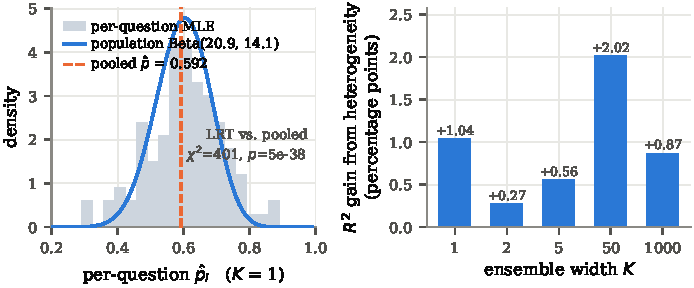
\includegraphics[width=\textwidth]{heterogeneity.pdf}
  \caption{Prompt-level heterogeneity. \textbf{Left:} per-question acceptance
  probabilities at $K=1$, the fitted population $\mathrm{Beta}(a,b)$, and the
  pooled estimate; the empirical spread is wider than the population because the
  per-question MLEs carry estimation noise. \textbf{Right:} the resulting gain in
  histogram fit, recomputed against the same predictions used in
  Figure~\ref{fig:histbyk} and Table~\ref{tab:fit}. The gain is positive at
  every width but not monotone in $K$.}
  \label{fig:heterogeneity}
\end{figure}

\subsection{Self-verification}

Dropping the base model entirely and verifying against the proposal model's own
autoregressive prediction is attractive --- one set of weights, no second model
--- and it does raise tokens per call ($3.86$ exact, $6.45$ with nucleus
$\theta = 0.8$). But faithfulness collapses: $\bar q = 65.9$ for exact
self-verification and $24.7$ with nucleus. This is expected rather than
surprising. Self-verification removes the only reference to the distribution we
are asking the output to match, so the generation is free to drift, and the
metric that detects drift duly does. Self-verification is the right tool when the
goal is a fast standalone generator, and the wrong one when the goal is to
accelerate a \emph{specific} base model.

\section{Related work}

Speculative decoding proposes tokens with a cheap drafter and verifies them
against the target model with a distribution-preserving acceptance
rule~\citep{leviathan2023speculative,chen2023accelerating}; our exact rule is its
analogue under shared auxiliaries. A large family of methods makes the drafter
cheaper or better: extra decoding heads~\citep{stern2018blockwise,cai2024medusa},
sequentially dependent heads~\citep{ankner2024hydra}, feature-space
drafting with dynamic draft trees~\citep{li2024eagle,li2024eagle2},
Jacobi-style parallel decoding~\citep{fu2024lookahead}, and retrieval from the
prompt~\citep{saxena2023pld}. Multi-token prediction has also been used as a
training objective in its own right~\citep{gloeckle2024multitoken}. All of these
inherit the acceptance rule rather than study it, and are benchmarked with
accepted-tokens-per-call and speedup~\citep{xia2024specbench} but not with a test
of distributional faithfulness. PTP~\citep{draxler2025ptp} supplies the proposal
mechanism we build on, along with Partial Quadratic Decoding; the connection
between auxiliary variables and inverse autoregressive
flows~\citep{kingma2016iaf} is noted there. Our branching model is a
zero-inflated, shared-frailty Galton--Watson process~\citep{athreya1972branching}.

\section{Conclusion}

Treating the acceptance rule as a design variable rather than a fixed detail
changes the picture of multi-token inference. Accepted-tokens-per-call,
wall-clock speedup, and faithfulness to the base model rank decoding rules
differently, and reporting only the first --- as is common --- can recommend a
configuration that is both slower and less faithful than the alternative. A
three-parameter branching model of the number of correct tokens per call captures
the per-call distribution across three orders of magnitude of proposal width, and
makes the proposal-geometry question an exactly solvable knapsack whose solution
also supplies the branch weights and branch values that Partial Quadratic
Decoding needs.

\paragraph{Limitations.}
All numbers are preliminary, single-seed, and from one model pair
(Vicuna-7B and one distilled student) on one GPU; the wall-clock conclusions in
particular are hardware- and implementation-specific, and the ensemble rules
would be read differently on hardware with spare parallel capacity. We evaluate
only first turns of Spec-Bench, which leaves no reference completion, so our
quality measures are all relative to the base model rather than to a ground
truth; a rule that drifts towards \emph{better} text than the base model's would
be penalized by $p_{\mathrm{align}}$ exactly as one that drifts towards worse. The
fitted $(\pizero, p, \rhoc)$ is depth-uniform and checkpoint-specific, and its
extrapolation degrades at $K = 1000$. The ratio-rule anomaly of
\S\ref{sec:exp:rules} is unresolved.

\bibliography{iclr2026_conference}
\bibliographystyle{iclr2026_conference}

\appendix
\section{All decoding configurations}

Table~\ref{tab:all} lists every configuration, sorted by wall-clock speedup.
Re-run variants of identical configurations are excluded, as are runs marked
superseded in the source tree. ``gzip'' is the compression ratio of the generated
text, a model-free repetition proxy; lower means more repetitive.

\begin{table}[h]
  \centering
  \caption{All $62$ decoding configurations, sorted by speedup. Preliminary.}
  \label{tab:all}
  \tiny
  {\setlength{\tabcolsep}{3pt}%
\begin{tabular}{llrrrrrr}
\toprule
run & family & \multicolumn{1}{c}{tok./call} & \multicolumn{1}{c}{ms/tok.} & \multicolumn{1}{c}{speedup} & \multicolumn{1}{c}{$\bar q$ (\%)} & \multicolumn{1}{c}{PPL} & \multicolumn{1}{c}{gzip} \\
\midrule
\texttt{ratio-p-0.5} & ratio & 15.20 & 5.8 & 9.70$\times$ & 49.16 & 240.22 & 0.226 \\
\texttt{conf-p-0.1} & student confidence & 15.59 & 9.8 & 5.76$\times$ & 43.36 & 124.70 & 0.125 \\
\texttt{thresh-0.0000000001} & teacher threshold & 17.23 & 13.6 & 4.13$\times$ & 44.41 & 96.82 & 0.318 \\
\texttt{first\_4} & accept-$k$ & 4.00 & 16.1 & 3.50$\times$ & 47.34 & 31.99 & 0.310 \\
\texttt{ratio-p-0.1} & ratio & 6.65 & 18.5 & 3.06$\times$ & 45.10 & 19.04 & 0.520 \\
\texttt{ptp\_self} & self-verified & 3.50 & 24.7 & 2.29$\times$ & 66.21 & 1.61 & 0.550 \\
\texttt{seq-ptp-topp-self-0.99-tok} & self-verified & 12.21 & 25.6 & 2.21$\times$ & 15.94 & 91.95 & 0.471 \\
\texttt{seq-ptp-self-aux} & self-verified & 6.45 & 29.0 & 1.94$\times$ & 53.88 & 5.45 & 0.479 \\
\texttt{ratio-10000} & ratio & 2.61 & 30.9 & 1.83$\times$ & 70.33 & 1.57 & 0.721 \\
\texttt{conf-p-0.25} & student confidence & 5.84 & 31.0 & 1.82$\times$ & 50.57 & 57399.95 & 0.363 \\
\texttt{tmp\_seq-ptp-topp-0.99} & nucleus & 5.04 & 31.0 & 1.82$\times$ & 65.83 & 1.67 & 0.641 \\
\texttt{ratio-10} & ratio & 2.62 & 31.0 & 1.82$\times$ & 70.12 & 1.57 & 0.717 \\
\texttt{first\_2} & accept-$k$ & 2.00 & 31.7 & 1.78$\times$ & 49.29 & 40.92 & 0.515 \\
\texttt{ratio-2} & ratio & 2.49 & 32.3 & 1.75$\times$ & 69.81 & 1.58 & 0.727 \\
\texttt{ptp} & exact & 2.39 & 32.7 & 1.73$\times$ & 84.51 & 1.19 & 0.685 \\
\texttt{tmp\_seq-ptp-topp-0.98} & nucleus & 4.30 & 33.2 & 1.70$\times$ & 67.58 & 1.56 & 0.671 \\
\texttt{ratio-p-0.01} & ratio & 2.36 & 33.9 & 1.66$\times$ & 62.33 & 1.83 & 0.736 \\
\texttt{ratio-p-0.001} & ratio & 2.35 & 34.1 & 1.66$\times$ & 69.56 & 1.59 & 0.728 \\
\texttt{ratio} & ratio & 2.35 & 34.3 & 1.65$\times$ & 69.94 & 1.58 & 0.726 \\
\texttt{tmp\_seq-ptp-topp-0.95} & nucleus & 3.96 & 34.7 & 1.62$\times$ & 70.99 & 1.46 & 0.687 \\
\texttt{ratio\_g} & ratio & 2.31 & 34.9 & 1.62$\times$ & 71.52 & 1.50 & 0.686 \\
\texttt{tmp\_seq-ptp-topp-0.9} & nucleus & 3.88 & 35.4 & 1.59$\times$ & 74.09 & 1.40 & 0.705 \\
\texttt{thresh-0.00001} & teacher threshold & 5.77 & 35.6 & 1.58$\times$ & 65.05 & 1.71 & 0.588 \\
\texttt{seq-ptp-topp-self-0.9-tok} & self-verified & 8.20 & 35.9 & 1.57$\times$ & 26.57 & 63.95 & 0.475 \\
\texttt{tmp\_seq-ptp-topp-0.5} & nucleus & 3.62 & 38.0 & 1.48$\times$ & 75.53 & 1.39 & 0.707 \\
\texttt{tmp\_seq-ptp-topp-self-0.8-tok} & self-verified & 6.45 & 39.8 & 1.42$\times$ & 24.66 & 38.70 & 0.537 \\
\texttt{first\_1.5} & accept-$k$ & 1.50 & 41.9 & 1.35$\times$ & 35.54 & 18.19 & 0.742 \\
\texttt{thresh-0.01} & teacher threshold & 3.93 & 42.4 & 1.33$\times$ & 77.75 & 1.31 & 0.671 \\
\texttt{tmp\_seq-ptp-topp-self-0.5-tok} & self-verified & 5.12 & 44.4 & 1.27$\times$ & 29.58 & 52.51 & 0.535 \\
\texttt{thresh-0.1} & teacher threshold & 3.58 & 46.0 & 1.23$\times$ & 83.16 & 1.21 & 0.672 \\
\texttt{seq-ratio} & ratio & 3.43 & 48.1 & 1.17$\times$ & 83.53 & 1.21 & 0.689 \\
\texttt{tmp\_seq-ptp-topp-choice-5-0.98-bayes-p} & nucleus + ensemble & 4.38 & 48.2 & 1.17$\times$ & 82.46 & 1.23 & 0.658 \\
\texttt{seq-ptp-self-tok} & self-verified & 3.86 & 49.9 & 1.13$\times$ & 65.92 & 1.60 & 0.555 \\
\texttt{first\_1.2} & accept-$k$ & 1.20 & 51.6 & 1.09$\times$ & 48.75 & 2.90 & 0.722 \\
\texttt{thresh-0.5} & teacher threshold & 3.22 & 52.3 & 1.08$\times$ & 85.26 & 1.18 & 0.678 \\
\texttt{tmp\_seq-ptp-topp-self-0.01-tok} & self-verified & 4.15 & 52.4 & 1.08$\times$ & 29.31 & 21.01 & 0.569 \\
\texttt{tmp\_seq-ptp-topp-self-0.1-tok} & self-verified & 3.98 & 52.6 & 1.07$\times$ & 28.96 & 24.87 & 0.564 \\
\texttt{seq-ratio\_g} & ratio & 3.21 & 53.0 & 1.06$\times$ & 81.29 & 1.25 & 0.687 \\
\texttt{seq-ptp} & exact & 3.63 & 55.3 & 1.02$\times$ & 84.71 & 1.19 & 0.687 \\
\texttt{tmp\_seq-ptp-topp-choice-5-0.98-bayes-conjugate} & nucleus + ensemble & 4.46 & 55.9 & 1.01$\times$ & 83.52 & 1.21 & 0.660 \\
\texttt{thresh-0.8} & teacher threshold & 2.95 & 56.1 & 1.00$\times$ & 84.43 & 1.19 & 0.684 \\
\texttt{ar} & autoregressive & 1.00 & 56.4 & 1.00$\times$ & 84.15 & 1.20 & 0.705 \\
\texttt{tmp\_seq-ptp-topp-choice-5-0.98} & nucleus + ensemble & 4.32 & 57.4 & 0.98$\times$ & 82.92 & 1.22 & 0.671 \\
\texttt{thresh-0.9} & teacher threshold & 2.81 & 60.8 & 0.93$\times$ & 84.44 & 1.19 & 0.687 \\
\texttt{first\_1} & accept-$k$ & 1.00 & 61.4 & 0.92$\times$ & 84.73 & 1.19 & 0.686 \\
\texttt{conf-p-0.5} & student confidence & 2.01 & 69.4 & 0.81$\times$ & 41.42 & 17.03 & 0.512 \\
\texttt{conf-p-0.8} & student confidence & 1.48 & 86.8 & 0.65$\times$ & 56.78 & 2.24 & 0.675 \\
\texttt{conf-p-0.9} & student confidence & 1.34 & 92.7 & 0.61$\times$ & 64.95 & 1.77 & 0.679 \\
\texttt{conf-p-0.95} & student confidence & 1.27 & 101.1 & 0.56$\times$ & 70.23 & 1.58 & 0.688 \\
\texttt{tmp\_seq-ptp-topp-choice-50-self-0.8-tok} & self-verified & 5.98 & 111.1 & 0.51$\times$ & 73.74 & 1.40 & 0.483 \\
\texttt{tmp\_seq-ptp-topp-choice-50-self-0.5-tok} & self-verified & 5.70 & 116.6 & 0.48$\times$ & 73.70 & 1.41 & 0.502 \\
\texttt{tmp\_ptp-topp-choice-50-self-0.5} & self-verified & 3.10 & 129.3 & 0.44$\times$ & 66.38 & 1.64 & 0.484 \\
\texttt{tmp\_seq-ptp-topp-choice-50-0.98} & nucleus + ensemble & 4.74 & 140.4 & 0.40$\times$ & 82.97 & 1.22 & 0.680 \\
\texttt{tmp\_seq-ptp-topp-choice-50-self-0.98-tok} & self-verified & 6.07 & 145.2 & 0.39$\times$ & 73.06 & 1.41 & 0.490 \\
\texttt{tmp\_seq-ptp-topp-choice-50-0.98-bayes-conjugate} & nucleus + ensemble & 4.77 & 159.8 & 0.35$\times$ & 82.02 & 1.23 & 0.685 \\
\texttt{tmp\_seq-ptp-topp-choice-50-self-0.8-bayes-conjugate-tok} & self-verified & 6.03 & 179.0 & 0.32$\times$ & 76.04 & 1.36 & 0.456 \\
\texttt{tmp\_seq-ptp-topp-choice-50-0.98-bayes-p} & nucleus + ensemble & 4.60 & 182.1 & 0.31$\times$ & 81.88 & 1.24 & 0.691 \\
\texttt{tmp\_seq-ptp-topp-choice-50-self-0.8-bayes-p-tok} & self-verified & 5.77 & 201.8 & 0.28$\times$ & 74.29 & 1.39 & 0.485 \\
\texttt{tmp\_seq-ptp-topp-choice-50-self-0.8-phead-tok} & self-verified & 3.45 & 325.4 & 0.17$\times$ & 74.48 & 1.39 & 0.512 \\
\bottomrule
\end{tabular}
}
\end{table}

\end{document}
